\documentclass{standalone}
\usepackage{tikz}
\usetikzlibrary{patterns, positioning}
\usepackage[sfdefault]{ClearSans} %% option 'sfdefault' activates Clear Sans as the default text font
\usepackage[T1]{fontenc}

\begin{document}
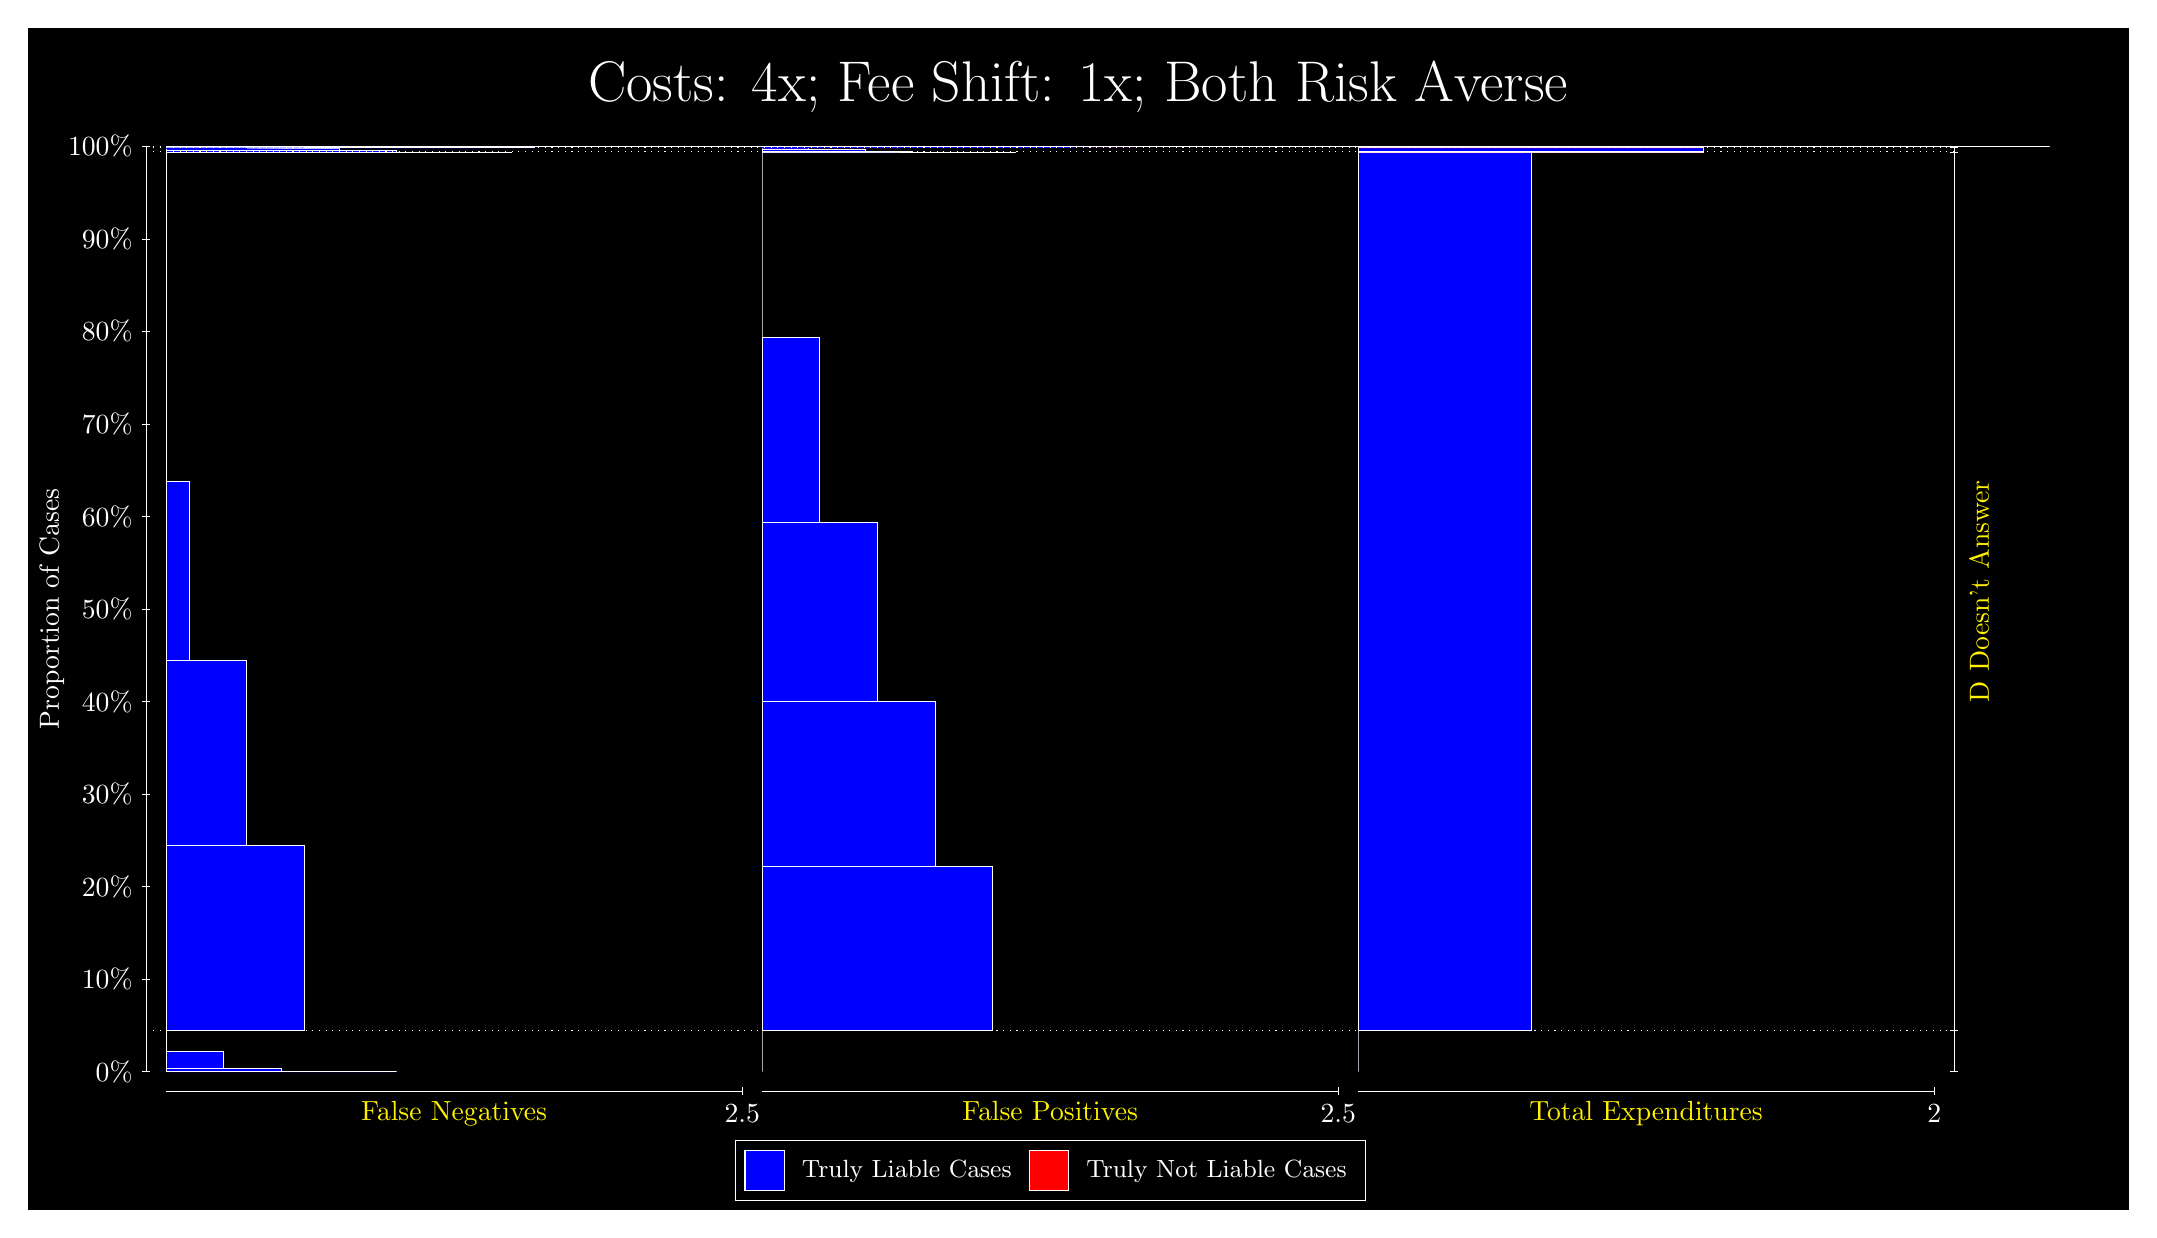
\begin{tikzpicture}
\draw[fill=black] (0,0) rectangle (26.667,15);
\draw[text=white] (0,13.5) rectangle (26.667,15) node[midway] {\huge Costs: 4x; Fee Shift: 1x; Both Risk Averse};
\draw[white, very thin] (1.5,1.75) -- (1.5,13.5);
\node[rotate=90, text=white, anchor=center] at (0.3, 7.625) {Proportion of Cases};
\draw[white, very thin] (1.45,1.75) -- (1.55,1.75);
\node[text=white, anchor=east] at (1.45, 1.75) {0\%};
\draw[white, very thin] (1.45,2.925) -- (1.55,2.925);
\node[text=white, anchor=east] at (1.45, 2.925) {10\%};
\draw[white, very thin] (1.45,4.1) -- (1.55,4.1);
\node[text=white, anchor=east] at (1.45, 4.1) {20\%};
\draw[white, very thin] (1.45,5.275) -- (1.55,5.275);
\node[text=white, anchor=east] at (1.45, 5.275) {30\%};
\draw[white, very thin] (1.45,6.45) -- (1.55,6.45);
\node[text=white, anchor=east] at (1.45, 6.45) {40\%};
\draw[white, very thin] (1.45,7.625) -- (1.55,7.625);
\node[text=white, anchor=east] at (1.45, 7.625) {50\%};
\draw[white, very thin] (1.45,8.8) -- (1.55,8.8);
\node[text=white, anchor=east] at (1.45, 8.8) {60\%};
\draw[white, very thin] (1.45,9.975) -- (1.55,9.975);
\node[text=white, anchor=east] at (1.45, 9.975) {70\%};
\draw[white, very thin] (1.45,11.15) -- (1.55,11.15);
\node[text=white, anchor=east] at (1.45, 11.15) {80\%};
\draw[white, very thin] (1.45,12.325) -- (1.55,12.325);
\node[text=white, anchor=east] at (1.45, 12.325) {90\%};
\draw[white, very thin] (1.45,13.5) -- (1.55,13.5);
\node[text=white, anchor=east] at (1.45, 13.5) {100\%};

\draw[white, very thin] (24.457,1.75) -- (24.457,13.5);
\draw[white, very thin] (24.407,1.75) -- (24.507,1.75);
\node[anchor=west] at (24.407, 1.75) {};
\draw[white, very thin] (24.407,2.2721) -- (24.507,2.2721);
\node[anchor=west] at (24.407, 2.2721) {};
\draw[white, very thin] (24.407,13.429) -- (24.507,13.429);
\node[anchor=west] at (24.407, 13.429) {};
\draw[white, very thin] (24.407,13.484) -- (24.507,13.484);
\node[anchor=west] at (24.407, 13.484) {};
\draw[white, very thin] (24.407,13.496) -- (24.507,13.496);
\node[anchor=west] at (24.407, 13.496) {};
\draw[white, very thin] (24.407,13.5) -- (24.507,13.5);
\node[anchor=west] at (24.407, 13.5) {};
\draw[white, very thin] (24.407,13.5) -- (24.507,13.5);
\node[anchor=west] at (24.407, 13.5) {};

\draw[white, very thin, fill=blue] (1.75,1.75) rectangle (4.6775,1.75);
\draw[white, very thin, fill=blue] (1.75,1.75) rectangle (3.9457,1.7504);
\draw[white, very thin, fill=blue] (1.75,1.7504) rectangle (3.2138,1.7918);
\draw[white, very thin, fill=blue] (1.75,1.7918) rectangle (2.4819,2.0114);
\draw[white, very thin, fill=red] (1.75,2.0114) rectangle (1.75,2.0114);
\draw[white, very thin, fill=blue] (1.75,2.0114) rectangle (1.75,2.2721);
\draw[white, very thin, fill=blue] (1.75,2.2721) rectangle (3.5065,4.622);
\draw[white, very thin, fill=blue] (1.75,4.622) rectangle (2.7746,6.9713);
\draw[white, very thin, fill=blue] (1.75,6.9713) rectangle (2.0428,9.2451);
\draw[white, very thin, fill=red] (1.75,9.2451) rectangle (1.75,9.2451);
\draw[white, very thin, fill=blue] (1.75,9.2451) rectangle (1.75,13.429);
\draw[white, very thin, fill=blue] (1.75,13.429) rectangle (6.1413,13.429);
\draw[white, very thin, fill=blue] (1.75,13.429) rectangle (5.8486,13.429);
\draw[white, very thin, fill=blue] (1.75,13.429) rectangle (5.5558,13.429);
\draw[white, very thin, fill=blue] (1.75,13.429) rectangle (5.4094,13.43);
\draw[white, very thin, fill=blue] (1.75,13.43) rectangle (5.2631,13.43);
\draw[white, very thin, fill=blue] (1.75,13.43) rectangle (5.1167,13.43);
\draw[white, very thin, fill=blue] (1.75,13.43) rectangle (4.9703,13.43);
\draw[white, very thin, fill=blue] (1.75,13.43) rectangle (4.8239,13.43);
\draw[white, very thin, fill=blue] (1.75,13.43) rectangle (4.6775,13.448);
\draw[white, very thin, fill=blue] (1.75,13.448) rectangle (4.5312,13.448);
\draw[white, very thin, fill=blue] (1.75,13.448) rectangle (4.3848,13.451);
\draw[white, very thin, fill=blue] (1.75,13.451) rectangle (4.2384,13.451);
\draw[white, very thin, fill=blue] (1.75,13.451) rectangle (4.092,13.453);
\draw[white, very thin, fill=blue] (1.75,13.453) rectangle (3.9457,13.477);
\draw[white, very thin, fill=blue] (1.75,13.477) rectangle (3.7993,13.477);
\draw[white, very thin, fill=blue] (1.75,13.477) rectangle (3.6529,13.48);
\draw[white, very thin, fill=blue] (1.75,13.48) rectangle (3.5065,13.481);
\draw[white, very thin, fill=blue] (1.75,13.481) rectangle (3.3602,13.483);
\draw[white, very thin, fill=blue] (1.75,13.483) rectangle (3.2138,13.483);
\draw[white, very thin, fill=blue] (1.75,13.483) rectangle (3.0674,13.483);
\draw[white, very thin, fill=blue] (1.75,13.483) rectangle (2.921,13.483);
\draw[white, very thin, fill=blue] (1.75,13.483) rectangle (2.7746,13.484);
\draw[white, very thin, fill=blue] (1.75,13.484) rectangle (2.6283,13.484);
\draw[white, very thin, fill=blue] (1.75,13.484) rectangle (2.3355,13.484);
\draw[white, very thin, fill=blue] (1.75,13.484) rectangle (2.0428,13.484);
\draw[white, very thin, fill=red] (1.75,13.484) rectangle (1.75,13.484);
\draw[white, very thin, fill=blue] (1.75,13.484) rectangle (6.4341,13.484);
\draw[white, very thin, fill=blue] (1.75,13.484) rectangle (5.7022,13.484);
\draw[white, very thin, fill=blue] (1.75,13.484) rectangle (4.9703,13.491);
\draw[white, very thin, fill=blue] (1.75,13.491) rectangle (4.2384,13.496);
\draw[white, very thin, fill=blue] (1.75,13.496) rectangle (3.5065,13.496);
\draw[white, very thin, fill=red] (1.75,13.496) rectangle (1.75,13.496);
\draw[white, very thin, fill=blue] (1.75,13.496) rectangle (3.5065,13.496);
\draw[white, very thin, fill=blue] (1.75,13.496) rectangle (2.7746,13.496);
\draw[white, very thin, fill=blue] (1.75,13.496) rectangle (2.0428,13.499);
\draw[white, very thin, fill=red] (1.75,13.499) rectangle (1.75,13.499);
\draw[white, very thin, fill=blue] (1.75,13.499) rectangle (1.75,13.5);
\draw[white, very thin, fill=blue] (1.75,13.5) rectangle (11.704,13.5);
\draw[white, very thin, fill=blue] (1.75,13.5) rectangle (10.972,13.5);
\draw[white, very thin, fill=blue] (1.75,13.5) rectangle (10.24,13.5);
\draw[white, very thin, fill=blue] (1.75,13.5) rectangle (9.508,13.5);
\draw[white, very thin, fill=blue] (1.75,13.5) rectangle (8.7761,13.5);
\draw[white, very thin, fill=blue] (1.75,13.5) rectangle (8.0442,13.5);
\draw[white, very thin, fill=blue] (1.75,13.5) rectangle (3.9457,13.5);
\draw[white, very thin, fill=blue] (1.75,13.5) rectangle (3.2138,13.5);
\draw[white, very thin, fill=blue] (1.75,13.5) rectangle (2.4819,13.5);
\draw[white, very thin, fill=red] (1.75,13.5) rectangle (1.75,13.5);
\draw[white, very thin, fill=blue] (1.75,13.5) rectangle (1.75,13.5);
\draw[white, very thin, fill=red] (9.3189,1.75) rectangle (9.3189,1.75);
\draw[white, very thin, fill=blue] (9.3189,1.75) rectangle (9.3189,2.2721);
\draw[white, very thin, fill=red] (9.3189,2.2721) rectangle (12.246,2.2721);
\draw[white, very thin, fill=blue] (9.3189,2.2721) rectangle (12.246,4.361);
\draw[white, very thin, fill=blue] (9.3189,4.361) rectangle (11.515,6.4565);
\draw[white, very thin, fill=blue] (9.3189,6.4565) rectangle (10.783,8.7302);
\draw[white, very thin, fill=blue] (9.3189,8.7302) rectangle (10.051,11.08);
\draw[white, very thin, fill=blue] (9.3189,11.08) rectangle (9.3189,13.429);
\draw[white, very thin, fill=red] (9.3189,13.429) rectangle (12.539,13.429);
\draw[white, very thin, fill=blue] (9.3189,13.429) rectangle (12.539,13.429);
\draw[white, very thin, fill=red] (9.3189,13.429) rectangle (12.246,13.429);
\draw[white, very thin, fill=blue] (9.3189,13.429) rectangle (12.246,13.429);
\draw[white, very thin, fill=red] (9.3189,13.429) rectangle (11.954,13.429);
\draw[white, very thin, fill=blue] (9.3189,13.429) rectangle (11.954,13.429);
\draw[white, very thin, fill=blue] (9.3189,13.429) rectangle (11.807,13.43);
\draw[white, very thin, fill=red] (9.3189,13.43) rectangle (11.661,13.43);
\draw[white, very thin, fill=blue] (9.3189,13.43) rectangle (11.661,13.43);
\draw[white, very thin, fill=blue] (9.3189,13.43) rectangle (11.515,13.43);
\draw[white, very thin, fill=red] (9.3189,13.43) rectangle (11.368,13.43);
\draw[white, very thin, fill=blue] (9.3189,13.43) rectangle (11.368,13.43);
\draw[white, very thin, fill=blue] (9.3189,13.43) rectangle (11.222,13.433);
\draw[white, very thin, fill=blue] (9.3189,13.433) rectangle (11.075,13.433);
\draw[white, very thin, fill=blue] (9.3189,13.433) rectangle (10.929,13.436);
\draw[white, very thin, fill=blue] (9.3189,13.436) rectangle (10.783,13.436);
\draw[white, very thin, fill=blue] (9.3189,13.436) rectangle (10.636,13.46);
\draw[white, very thin, fill=blue] (9.3189,13.46) rectangle (10.49,13.463);
\draw[white, very thin, fill=blue] (9.3189,13.463) rectangle (10.344,13.463);
\draw[white, very thin, fill=blue] (9.3189,13.463) rectangle (10.197,13.465);
\draw[white, very thin, fill=blue] (9.3189,13.465) rectangle (10.051,13.465);
\draw[white, very thin, fill=blue] (9.3189,13.465) rectangle (9.9044,13.484);
\draw[white, very thin, fill=blue] (9.3189,13.484) rectangle (9.758,13.484);
\draw[white, very thin, fill=blue] (9.3189,13.484) rectangle (9.6116,13.484);
\draw[white, very thin, fill=blue] (9.3189,13.484) rectangle (9.4652,13.484);
\draw[white, very thin, fill=blue] (9.3189,13.484) rectangle (9.3189,13.484);
\draw[white, very thin, fill=red] (9.3189,13.484) rectangle (11.075,13.484);
\draw[white, very thin, fill=blue] (9.3189,13.484) rectangle (11.075,13.484);
\draw[white, very thin, fill=blue] (9.3189,13.484) rectangle (10.344,13.489);
\draw[white, very thin, fill=blue] (9.3189,13.489) rectangle (9.6116,13.496);
\draw[white, very thin, fill=blue] (9.3189,13.496) rectangle (9.3189,13.496);
\draw[white, very thin, fill=red] (9.3189,13.496) rectangle (14.003,13.496);
\draw[white, very thin, fill=blue] (9.3189,13.496) rectangle (14.003,13.496);
\draw[white, very thin, fill=blue] (9.3189,13.496) rectangle (13.271,13.497);
\draw[white, very thin, fill=blue] (9.3189,13.497) rectangle (12.539,13.5);
\draw[white, very thin, fill=blue] (9.3189,13.5) rectangle (11.807,13.5);
\draw[white, very thin, fill=blue] (9.3189,13.5) rectangle (11.075,13.5);
\draw[white, very thin, fill=red] (9.3189,13.5) rectangle (19.273,13.5);
\draw[white, very thin, fill=blue] (9.3189,13.5) rectangle (19.273,13.5);
\draw[white, very thin, fill=red] (9.3189,13.5) rectangle (18.541,13.5);
\draw[white, very thin, fill=blue] (9.3189,13.5) rectangle (18.541,13.5);
\draw[white, very thin, fill=red] (9.3189,13.5) rectangle (17.809,13.5);
\draw[white, very thin, fill=blue] (9.3189,13.5) rectangle (17.809,13.5);
\draw[white, very thin, fill=red] (9.3189,13.5) rectangle (17.077,13.5);
\draw[white, very thin, fill=blue] (9.3189,13.5) rectangle (17.077,13.5);
\draw[white, very thin, fill=blue] (9.3189,13.5) rectangle (16.345,13.5);
\draw[white, very thin, fill=blue] (9.3189,13.5) rectangle (15.613,13.5);
\draw[white, very thin, fill=blue] (9.3189,13.5) rectangle (14.881,13.5);
\draw[white, very thin, fill=blue] (9.3189,13.5) rectangle (14.149,13.5);
\draw[white, very thin, fill=red] (9.3189,13.5) rectangle (10.051,13.5);
\draw[white, very thin, fill=blue] (9.3189,13.5) rectangle (10.051,13.5);
\draw[white, very thin, fill=red] (9.3189,13.5) rectangle (9.3189,13.5);
\draw[white, very thin, fill=blue] (9.3189,13.5) rectangle (9.3189,13.5);
\draw[white, very thin, fill=red] (16.888,1.75) rectangle (16.888,1.75);
\draw[white, very thin, fill=blue] (16.888,1.75) rectangle (16.888,2.2721);
\draw[white, very thin, fill=red] (16.888,2.2721) rectangle (19.083,2.2721);
\draw[white, very thin, fill=blue] (16.888,2.2721) rectangle (19.083,13.429);
\draw[white, very thin, fill=red] (16.888,13.429) rectangle (21.279,13.429);
\draw[white, very thin, fill=blue] (16.888,13.429) rectangle (21.279,13.431);
\draw[white, very thin, fill=red] (16.888,13.431) rectangle (21.279,13.431);
\draw[white, very thin, fill=blue] (16.888,13.431) rectangle (21.279,13.484);
\draw[white, very thin, fill=red] (16.888,13.484) rectangle (21.279,13.484);
\draw[white, very thin, fill=blue] (16.888,13.484) rectangle (21.279,13.496);
\draw[white, very thin, fill=red] (16.888,13.496) rectangle (21.279,13.496);
\draw[white, very thin, fill=blue] (16.888,13.496) rectangle (21.279,13.5);
\draw[white, very thin, fill=red] (16.888,13.5) rectangle (25.67,13.5);
\draw[white, very thin, fill=blue] (16.888,13.5) rectangle (25.67,13.5);
\draw[white, dotted] (1.5,2.2721) -- (24.457,2.2721);
\draw[white, dotted] (1.5,13.429) -- (24.457,13.429);
\draw[white, dotted] (1.5,13.484) -- (24.457,13.484);
\draw[white, dotted] (1.5,13.496) -- (24.457,13.496);
\draw[white, dotted] (1.5,13.5) -- (24.457,13.5);
\draw[white, very thin] (1.75,1.5) -- (9.0689,1.5);
\node[text=yellow, anchor=north] at (5.4094, 1.5) {False Negatives};
\draw[white, very thin] (9.0689,1.45) -- (9.0689,1.55);
\node[text=white, anchor=north] at (9.0689, 1.45) {2.5};

\draw[white, very thin] (9.3189,1.5) -- (16.638,1.5);
\node[text=yellow, anchor=north] at (12.978, 1.5) {False Positives};
\draw[white, very thin] (16.638,1.45) -- (16.638,1.55);
\node[text=white, anchor=north] at (16.638, 1.45) {2.5};

\draw[white, very thin] (16.888,1.5) -- (24.207,1.5);
\node[text=yellow, anchor=north] at (20.547, 1.5) {Total Expenditures};
\draw[white, very thin] (24.207,1.45) -- (24.207,1.55);
\node[text=white, anchor=north] at (24.207, 1.45) {2};


\node[text=yellow, centered, rotate=90] at (24.777, 7.8508) {D Doesn't Answer};





\draw (12.978300999999998,1.5) node[draw=none] (baseCoordinate) {};
\begin{scope}[align=center]
        \matrix[scale=0.5, draw=white, below=0.5cm of baseCoordinate, nodes={draw}, column sep=0.1cm]{
            \node[rectangle, draw, minimum width=0.5cm, minimum height=0.5cm, fill=blue] {}; &
            \node[draw=none, font=\small, text=white] (B) {Truly Liable Cases}; &
            \node[rectangle, draw, minimum width=0.5cm, minimum height=0.5cm, fill=red] {}; &
            \node[draw=none, font=\small, text=white] (B) {Truly Not Liable Cases}; \\
            };
\end{scope}

\end{tikzpicture}
\end{document}